\section{Mischer, Phasenregelkreise und Schrittgeneratoren}
\subsection{Phasenregelkreis}
\centering
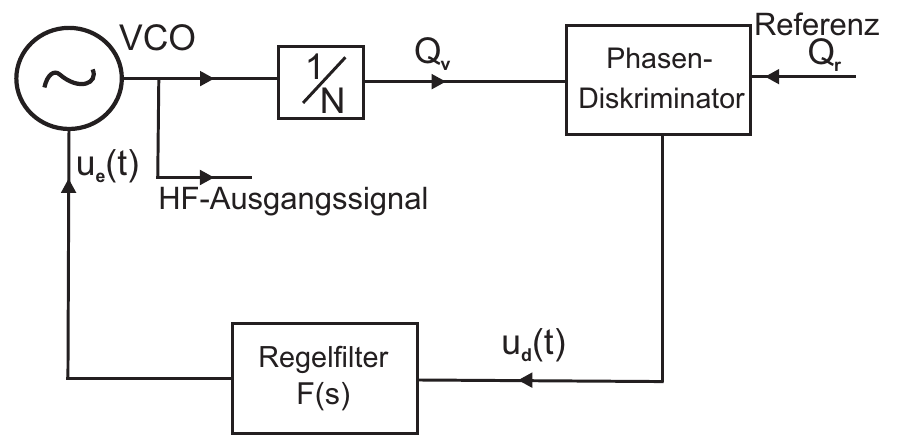
\includegraphics[width=.3\paperheight]{content/hfmess/pictures/pll_grundschaltung.png}
\textbf{Grundschaltung des PLLs}
\begin{itemize}
    \itemsep0pt
    \item \textbf{Ziel:} \textit{feste} Frequenzabstand zw. Signal- und LO-Frequenz einhalten
    \item Frequenzveränderliche VCO mit $f_v$ soll auf Referenz $f_r$ einrasten
    \item Nach dem einrasten gilt:
        \begin{equation*}
            f_v - f_r = 0\;\text{ oder }\;|f_v - f_r| = f_i
        \end{equation*}
    \begin{align*}
        &\parbox{2cm}{Verstärkung des offenen Regelkreises:} &V(s) = \dfrac{K_v K_d}{N} \dfrac{F(s)}{s}\\\\
        &\parbox{2cm}{Phase des VCO (Regelgröße):} &\Theta_v(s) = \dfrac{V(s)}{1 + V(s)}\Theta_r(s) = H(s)\Theta_r(s)\\
    \end{align*}
    \begin{align*}
        &K_d\;[V/\mathrm{rad}]: &\text{Steilheit des PDs}\\
        &K_v\;[\mathrm{rad}/Vs]: &\text{Abstimmsteilheit des VCO}\\
    \end{align*}
    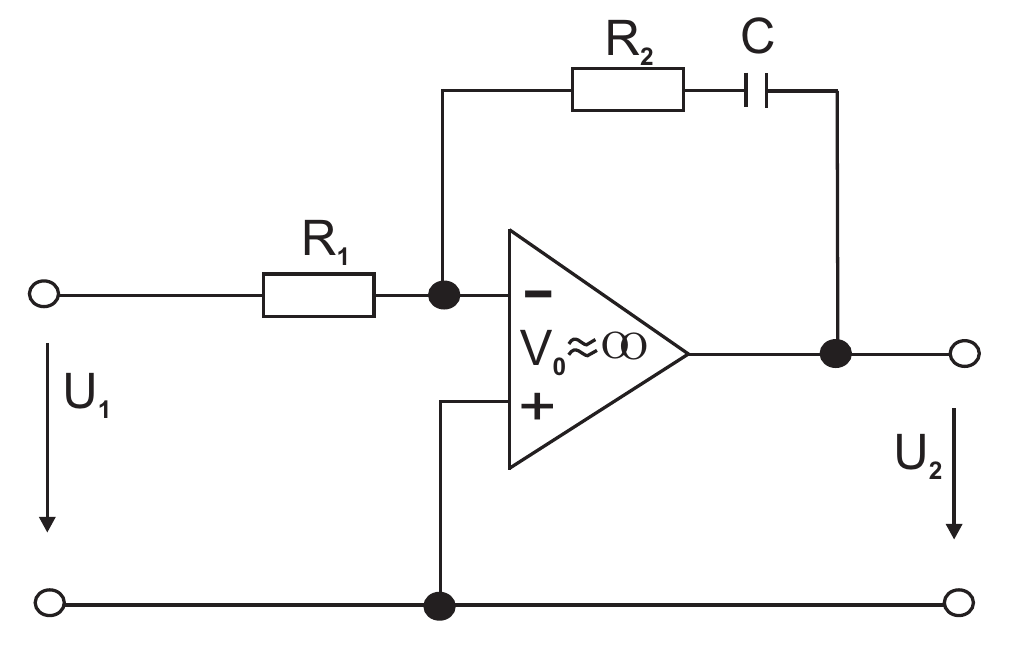
\includegraphics[width=.22\paperheight]{content/hfmess/pictures/pll_filter.png}\\
    \textbf{Beispiel: Aktive Regelfilter 1. Ordnung}
    \begin{align*}
        &F(s) = \dfrac{U_2}{U_1} = - \dfrac{s\tau_2 + 1}{s\tau_1},\\
        &\tau_i = R_i C, \quad i = 1,2
    \end{align*}
    \item Normalform von $\Theta_v$ und $V(s)$ mit akt. Regelfilter 1. Ordnung:
\end{itemize}
\begin{align*}
    &V(s) = \dfrac{2\zeta\omega_n s + \omega_n^2}{s^2},\\
    &H(s) = \dfrac{2\zeta\omega_n s + \omega_n^2}{s^2 + 2\zeta\omega_n s + \omega_n^2}\\
\end{align*}
\begin{equation*}
    \omega_n = \sqrt{\dfrac{K_v K_d}{\tau_1}}, \quad \zeta = \dfrac{1}{2}\tau_2\sqrt{\dfrac{K_v K_d}{\tau_1}} = \dfrac{1}{2}\tau_2 \omega_n
\end{equation*}

\subsection{Analoge und digitale Phasendiskriminatoren (PD)}
\begin{align*}
    \text{Referenz: } u_r(t) &= U_r \cos(\Omega t + \Theta_r)\\
    \text{VCO: } u_v(t) &= U_v \cos(\Omega t + \Theta_v)\\
    \text{Ausgang: } u_d(t) &= \dfrac{1}{2} U_r U_v  \cos(\Theta_r - \Theta_v)\\
        &+ \dfrac{1}{2} U_r U_v \cos(2\Omega t + \Theta_r + \Theta_v)\\
\end{align*}
\begin{itemize}
    \itemsep0pt
    \item Doppelt balancierte Mischer (\textbf{analoge} Produktmodulator) als PD:
        \begin{itemize}
            \itemsep0pt
            \item \textbf{Periodischer PD}: rastet erst ein, wenn Referenzfrequenz und VCO bis auf $\omega_n$ angenähert haben
            \item Es wird \textit{nicht} Seitenband-selektiv eingerastet
            \item Kennlinie ist nur in einem engen Bereich \textit{linear}
            \item Geringes Rauschen
            \item Höhere Betriebsfrequenz
        \end{itemize}
        \item Für \textit{periodische} PDs gilt:
            \begin{equation*}
                f_v - f_p = f_{\mathrm{ref}}\; \text{ oder }\; f_p - f_v = f_{\mathrm{ref}}
            \end{equation*}
        \item \textbf{Digitale} Realisierungen des PD:
            \begin{itemize}
                \itemsep0pt
                \item XOR-Gatter
                \item Flankengetriggerte FlipFlop
            \end{itemize}
\end{itemize}

\subsection{Phasen-Frequenz-Diskriminatoren (PFD)}
\begin{itemize}
    \itemsep0pt
    \item \textbf{Vorteil ggü. PDs:} PFDs können auch bei \textit{großen} Frequenzunterschieden ein definiertes Regelsignal liefern
    \item FlipFlop Schaltung als PFD:
        \begin{itemize}
            \itemsep0pt
            \item Für eine gute Regelung muss das Ausgangssignal $>2$ Werte annehmen
            \item Durch die analoge Differenzbildung am Ausgang kann $Q$ drei versch. Werte annehmen +1,0,-1
        \end{itemize}
\end{itemize}

\subsection{Schritt- und Synthesegeneratoren}
